\section{Koordinatensysteme \dcfirstauthorshort} \label{sec:ks}

%Um ein Modellauto steuern zu können, werden unter anderem die Informationen über den aktuellen Standort und den Zielpunkt, den das Fahrzeug ansteuern soll, benötigt. Die Trajektorie ist wiederum davon abhängig, an welcher Stelle sich die Fahrbahnmarkierungen befinden. 

Alle Positionen von Objekten im Raum können mit Entfernungen relativ zu entsprechenden \gls{acr:ks} beschrieben werden. Für die Beschreibung unseres \gls{glos:tucar}s auf dem Parcours und die Lage der Straßenlinien wurden vier kartesische, hierarchisch angeordnete \gls{acr:ks} festgelegt, welche in Abbildung~\ref{fig:grundlagen_kos} verdeutlicht werden. Auch wenn sich der Roboter natürlich im dreidimensionalen aufhält, reicht eine 2D-Beschreibung für unsere Anwendung aus. Die Testumgebung beinhaltet keinerlei Höhenunterschiede. So lassen sich alle zu beschreibenden Punkte im Raum auf die Straßenebene projizieren. 

\begin{figure}[h] % [htb]
  \centering
  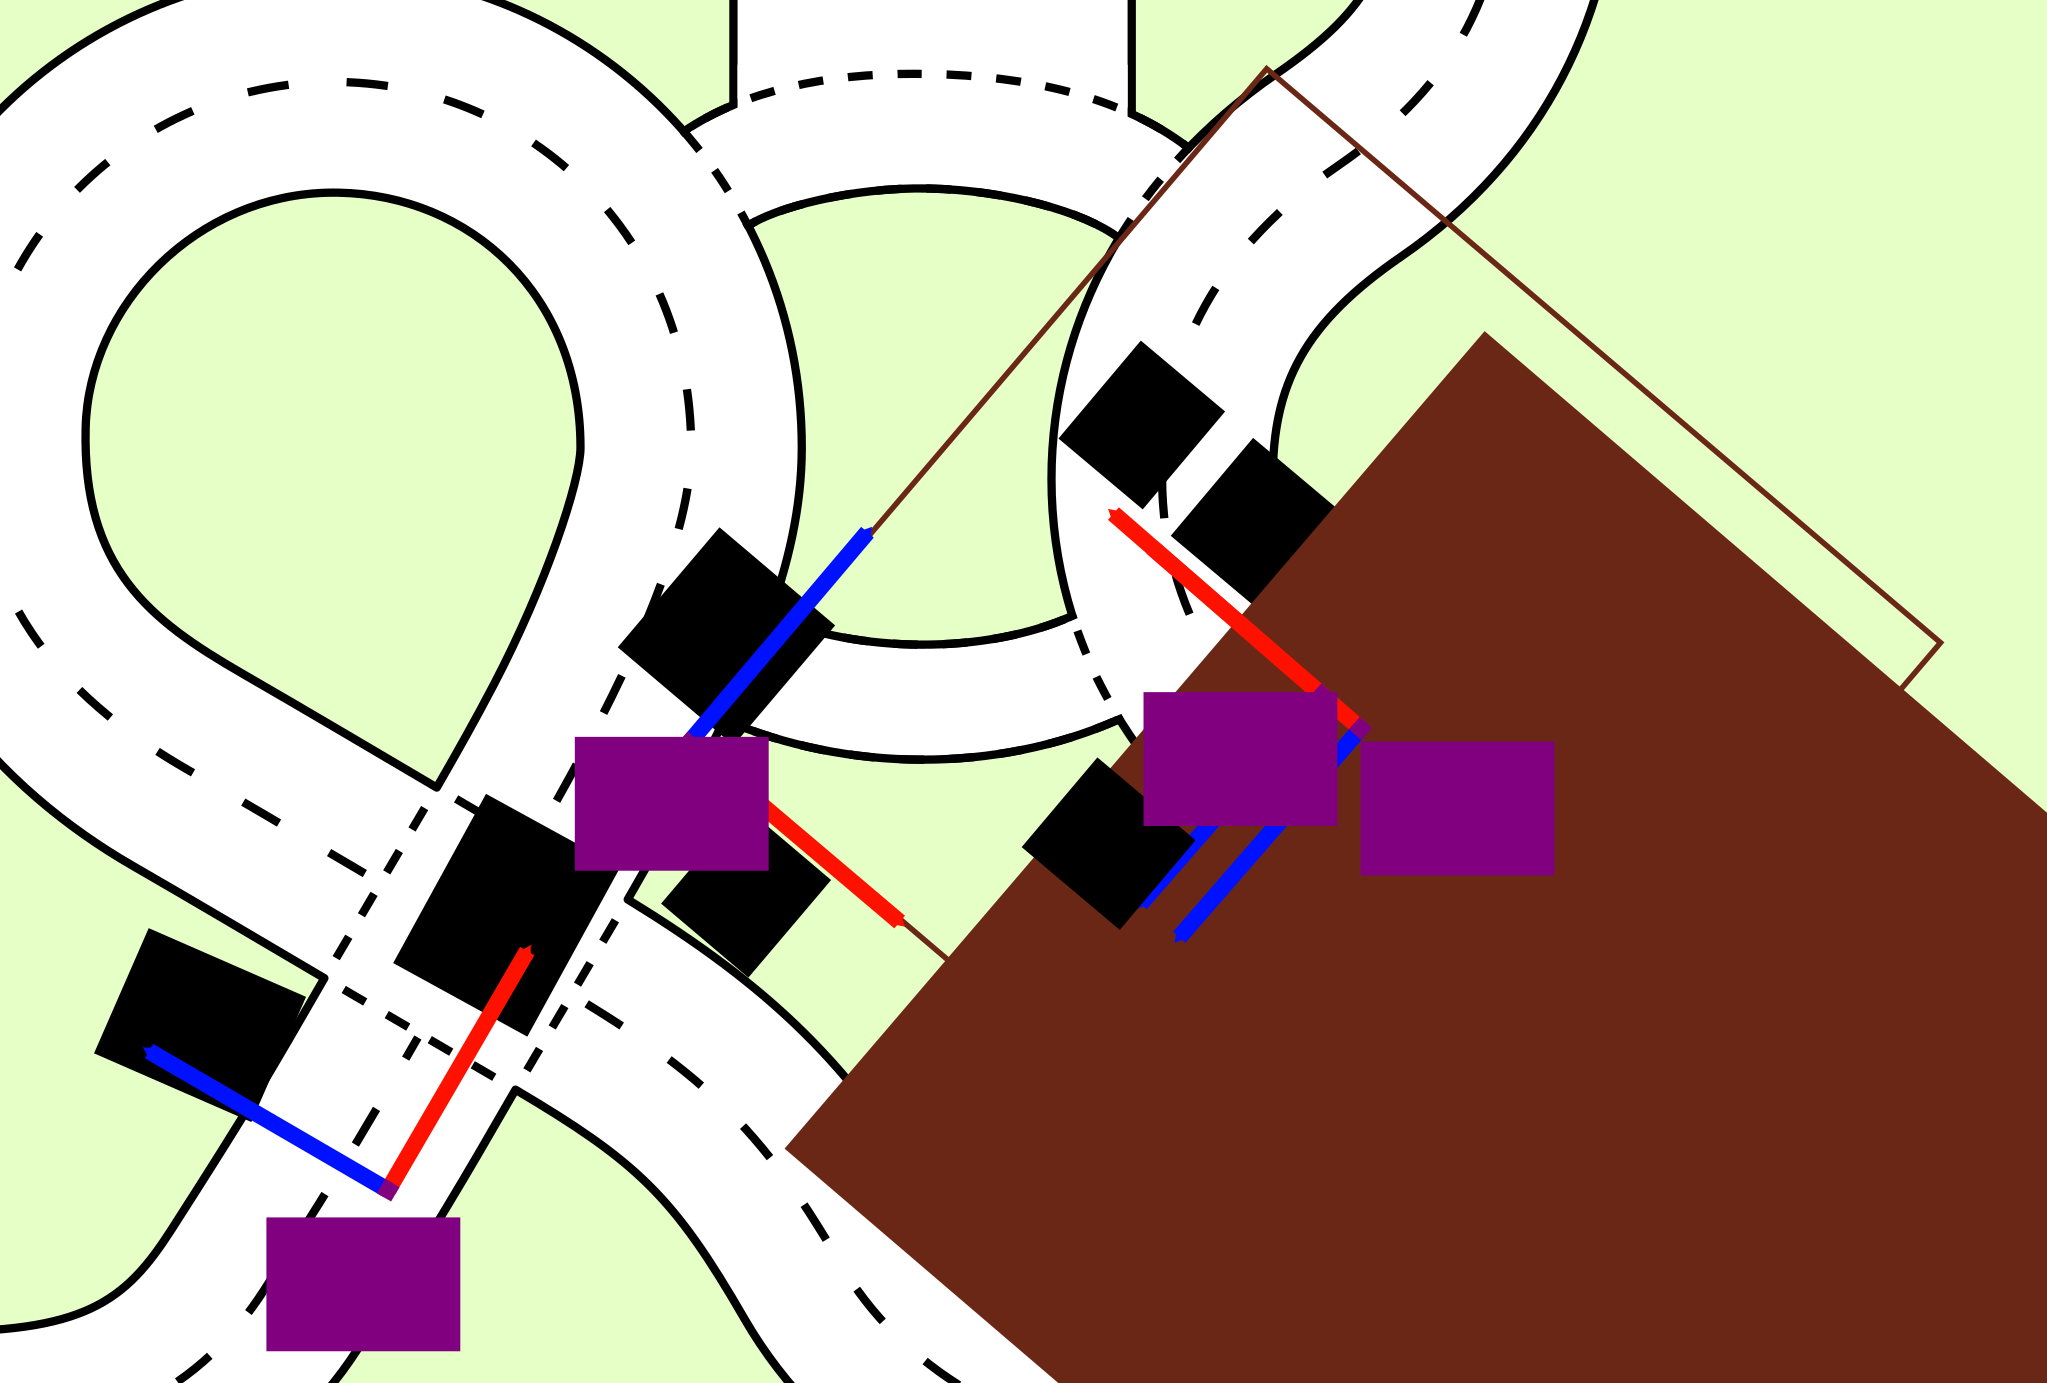
\includegraphics[width=0.9\textwidth]{grundlagen_kos.pdf}
  \caption{Alle eingeführten Koordinatensysteme im Überblick}
  \label{fig:grundlagen_kos}
\end{figure}

Das Weltkoordinatensystem \gls{lat:WeltKOS} bildet die Basis und ist an einem beliebigen Punkt des Szenarios verankert. Es dient zur Beschreibung der Pose des mobilen Roboters und der Linienpunkte in der Weltkarte. 

Die Pose bezeichnet den Zustandsvektor aus Position und Orientierung des Fahrzeugs in der Welt (siehe Gleichung~\eqref{eq:regelung_prinzip_pose}). Deren Lage bezeichnet das Roboterkoordinatensystem \gls{lat:RoboterKOS}, welches in der Hinterachse des Autos festgelegt ist. 

Damit sich die Pixelkoordinaten des Bildes nicht von der Matrixindizierung unterscheiden, wird das Bildkoordinatensystem \gls{lat:BildKOS} in die linke obere Ecke des entzerrten Fotos gelegt. So zeigt die \( {\gls{x}}^{\gls{lat:BildKOS}} \)-Achse in Richtung der Zeilen und die Spalten laufen mit der \( {\gls{y}}^{\gls{lat:BildKOS}} \)-Koordinate. 

Das Bild wird von der über dem Auto angebrachten Kamera aufgenommen. Die auf die Straßenebene projizierte Lage der Kamera wird als Kamerakoordinatensystem \gls{lat:CamKOS} festgelegt, welches die Verbindung zwischen Roboter- und Bildkoordinatensystem darstellt.

% Zwischenzeitlich hatten wir zusätzlich ein Linienkoordinatensystem \gls{lat:LinienKOS} festgelegt, welches so in der Bildecke platziert war, dass dessen \( {\gls{x}}^{\gls{lat:LinienKOS}} \)-Achse parallel zu der erwarteten Fahrbahnmarkierung verläuft, wenn das Auto auf einem geraden Abschnitt fährt. Der Grund dafür war die anfängliche Beschreibung der Linie mit einem Polynom dritten Grades (siehe Gleichung~\ref{eq:polynom3}) und die zuerst anders angedachte Orientierung der angebrachten Kamera. Dafür war es wichtig, dass die Fahrspur im \gls{acr:ks} keine Parallele zur Ordinate darstellt, da sie in diesem Fall schlecht durch ein Polynom hätte approximiert werden können. In Abbildung~\ref{fig:fahrspurerkennung_ransac_binarisieren} ist beispielsweise eine alte Kameraeinstellung zu sehen, in welcher das Linienkoordinatensystem zur Anwendung gekommen ist. 

Für die festgelegten \gls{acr:ks} gelten zwei zum Einsatz gekommene Einheiten. Punkte im Welt- und Roboterkoordinatensystem werden in Millimetern und im Kamera- und Bildkoordinatensystem in Pixeln beschrieben. Ein Pixel entspricht ungefähr 3,9 Millimetern.

\section{Koordinatentransformationen}

Die eben eingeführten Koordinatensysteme dienen der Darstellung jeweils dazu passender Objekte. Oft ist dagegen auch deren Beschreibung in anderen \gls{acr:ks} gefragt. Um beispielsweise in Roboterkoordinaten erkannten Hindernissen deren Position in der Weltkarte zuschreiben zu können, bedarf es einer Umrechnung. 

Für die Transformation von Punkten in ein anderes \gls{acr:ks} wird eine Verschiebung (Translation) in Richtung eines Translationsvektors \gls{lat:Translationsvektor}, eine Drehung mittels einer Rotationsmatrix \gls{lat:Rotationsmatrix} (Rotation) und gegebenenfalls eine Skalierung durchgeführt.
Mathematisch lassen sich \gls{lat:Translationsvektor}, \gls{lat:Rotationsmatrix} und die Skalierungsmatrix \gls{lat:Skalierungsmatrix} wie folgt darstellen \autocite[S.~26f]{corkeRoboticsVisionControl2017}, \autocite[S.~133]{nischwitzComputergrafik2011}.

% Formel für den Translationsvektor t
\begin{equation}
\gls{lat:Translationsvektor} = 
\begin{pmatrix}
\scl{t_x} 	\\
\scl{t_y} 	\\
\end{pmatrix}
, \qquad
% Formel für Rotationsmatrix
\gls{lat:Rotationsmatrix} = 
\begin{pmatrix}
\cos{\scl{\delta}} & -\sin{\scl{\delta}} 	\\
\sin{\scl{\delta}} & \cos{\scl{\delta}} 	\\
\end{pmatrix}
, \qquad
\gls{lat:Skalierungsmatrix} =
\begin{pmatrix}
\lambda_x 	& 0 		\\
0 			& \lambda_y 	\\
\end{pmatrix}
\end{equation} 

Da sich unser Roboter in der Darstellung nur im zweidimensionalen Raum bewegt, können Punkte lediglich in dieser Ebene rotiert werden (sprich: um die nicht vorhandene \gls{z}-Achse gedreht werden). 
Sind beispielsweise die Weltkoordinaten von Punkten im Roboterkoordinatensystem gesucht, so stellen \gls{lat:Translationsvektor} die Position und \( \scl{\delta} = \gls{gre:orientierung} \) die Orientierung des Modellfahrzeugs dar.
Eine Abbildung des Punktvektors \( \pnt{p}^{\gls{lat:RoboterKOS}} \) in das \gls{lat:WeltKOS}-\gls{acr:ks} könnte dann wie folgt aussehen:

% Formel Rotation und Translation  
\begin{equation}
\pnt{p}^{\gls{lat:WeltKOS}} =
\gls{lat:Skalierungsmatrix}^{\gls{lat:WeltKOS}\gls{lat:RoboterKOS}} \cdot \gls{lat:Rotationsmatrix}^{\gls{lat:WeltKOS}\gls{lat:RoboterKOS}} 
\cdot \pnt{p}^{\gls{lat:RoboterKOS}} + {\gls{lat:Translationsvektor}}^{\gls{lat:WeltKOS}}_{\gls{lat:RoboterKOS}}
\label{eq:RotTrans}
\end{equation}

%Die Matrix \gls{lat:Transformationsmatrix}, welche die Punkte \pnt{p} transformiert, sodass \gls{acr:zb}
%\( \pnt{p}^{\gls{lat:WeltKOS}} = \gls{lat:Transformationsmatrix}^{\gls{lat:WeltKOS}\gls{lat:RoboterKOS}} \cdot  \pnt{p}^{\gls{lat:RoboterKOS}} \) gilt, heißt homogene Transformationsmatrix und wird folgendermaßen aufgestellt:

Diese Kombination aus Rotation und Translation lässt sich ebenso in einer Matrix \gls{lat:Transformationsmatrix} zusammenfassen, sodass man anstatt Gleichung~\eqref{eq:RotTrans} auch folgendes schreiben kann.

\begin{equation}
\pnt{p}^{\gls{lat:WeltKOS}} = \gls{lat:Transformationsmatrix}^{\gls{lat:WeltKOS}\gls{lat:RoboterKOS}} 
\cdot \pnt{p}^{\gls{lat:RoboterKOS}} 
\end{equation}

Die Matrix \gls{lat:Transformationsmatrix} heißt homogene Transformationsmatrix und wird folgendermaßen aufgestellt \autocite[S.~26f]{corkeRoboticsVisionControl2017}:

% Formel für die Transformationsmatrix T
\begin{equation}
\gls{lat:Transformationsmatrix} = 
\begin{pmatrix}
\gls{lat:Skalierungsmatrix}\gls{lat:Rotationsmatrix} 	
&  \gls{lat:Translationsvektor}								\\
0 \quad 0 					& 1 							\\
\end{pmatrix}
=
\begin{pmatrix}
\lambda_x \cdot \cos{\scl{\delta}} 	& -\lambda_x \cdot \sin{\scl{\delta}}	& \scl{t_x} 	\\
\lambda_y \cdot \sin{\scl{\delta}} 	& \lambda_y \cdot \cos{\scl{\delta}} 	& \scl{t_y} 	\\
0 					& 0  					& 1 			\\
\end{pmatrix}
\end{equation}

So lassen sich jegliche Transformationen zwischen aufeinanderfolgenden \gls{acr:ks} realisieren, wenn die Parameter Rotationswinkel \(\delta\), Translationsvektor \gls{lat:Translationsvektor} und die Skalierungsfaktoren bekannt sind. Für uniforme Skalierungen gilt \( \lambda_x = \lambda_y \). Dabei ist eine Hierarchie\footnote{Unsere Koordinatensystemhierarchie: \(\gls{lat:WeltKOS} \rightarrow \gls{lat:RoboterKOS} \rightarrow \gls{lat:CamKOS} \rightarrow \gls{lat:BildKOS} \)} der \gls{acr:ks} sinnvoll, da sich z.B. die unbekannte Transformationsmatrix \(\gls{lat:Transformationsmatrix}^{\gls{lat:WeltKOS} \gls{lat:BildKOS}}\), welche Bildkoordinaten in Weltkoordinaten transformiert, durch Multiplikation bereits bekannter Matrizen ermitteln lässt. Es gilt: 

% Formel für die Hintereinanderausführung der Transformation
\begin{equation}
\gls{lat:Transformationsmatrix}^{\gls{lat:WeltKOS} \gls{lat:BildKOS}} = 
\gls{lat:Transformationsmatrix}^{\gls{lat:WeltKOS} \gls{lat:RoboterKOS}} \cdot
\gls{lat:Transformationsmatrix}^{\gls{lat:RoboterKOS} \gls{lat:CamKOS}} \cdot
\gls{lat:Transformationsmatrix}^{\gls{lat:CamKOS} \gls{lat:BildKOS}}
\end{equation}

Für die Transformation in umgekehrter Richtung kann die Inverse der homogenen Transformationsmatrix angewendet werden \( \left( \gls{lat:Transformationsmatrix}^{\gls{lat:BildKOS} \gls{lat:WeltKOS}} = {(\gls{lat:Transformationsmatrix}^{\gls{lat:WeltKOS} \gls{lat:BildKOS}})}^{-1} \right) \). Ein Beispiel für die Transformation des Punktes \( \pnt{p}^{\gls{lat:RoboterKOS}} \) in Weltkoordinaten sieht folglich so aus:

% Beispielformel
\begin{equation}
\pnt{p}^{\gls{lat:WeltKOS}} =
\gls{lat:Transformationsmatrix}^{\gls{lat:WeltKOS} \gls{lat:RoboterKOS}} \cdot 
\pnt{p}^{\gls{lat:RoboterKOS}} =
\begin{pmatrix}
\cos{30^\circ} 	& -\sin{30^\circ} 	& 420 	\\
\sin{30^\circ} 	& \cos{30^\circ} 	& 170 	\\
0 				& 0 				& 1 	\\
\end{pmatrix}
\cdot
\begin{pmatrix}
230 	\\
350 	\\
1   \\
\end{pmatrix}
=
\begin{pmatrix}
444,1858 	\\
588,1089 	\\
1    	\\
\end{pmatrix}
\end{equation}

